\section{Testbed Environment Description}
\label{sec:testbed}

We used Data Direct Networks' (DDN) SFA10K as the storage backend during this
evaluation. It consists of 200 SAS drives and 280 SATA drives, organized into
various RAID levels by two active-active RAID controllers. The exported RAID
groups by these controllers are driven by four hosts.
Each host has two InfiniBand (IB) QDR connections to the storage backend.
We used a single dualport Mellanox connectX IB card per host.
By our calculation, this setup can saturate SFA10K's maximum theoretical
throughput (\textasciitilde 12 GB/s). The connection diagram is illustrated in
Figure~\ref{fig:ddn-sfa10k}.

\begin{figure}[htb]
\centering
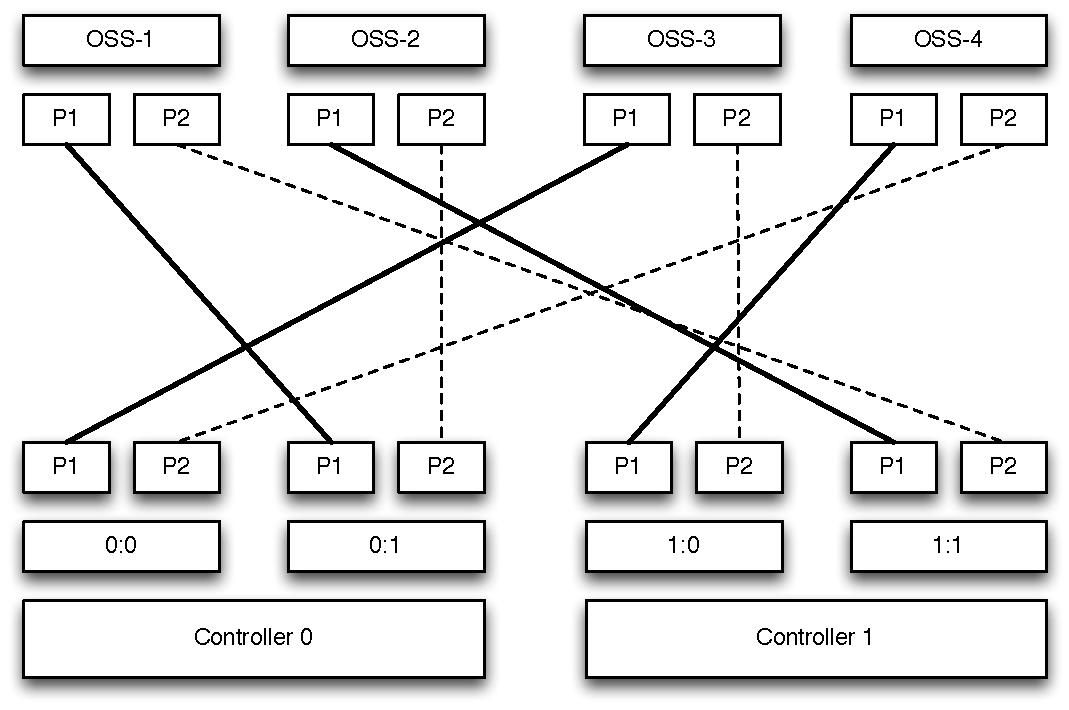
\includegraphics[width=3in]{figs/sfa10k}
\caption{DDN SFA10K hardware and host connection diagram}
\label{fig:ddn-sfa10k}
\end{figure}


Our Ceph testbed employs a collection of testing nodes. These nodes and their
roles are summarized in Table~\ref{tbl:ceph-test-nodes}. In the following
discussion, we use ``servers'', ``osd servers'', ``server hosts''
interchangably. We will emphasize with ``client'' prefix when we want to
distinguish it from above.

\begin{table}[!t]
\centering
\caption{Support nodes involved in Ceph testbed}
\label{tbl:ceph-test-nodes}
    \begin{tabular}{ll}
    \hline
    Node & Role \\
    \hline
    tick-mds1 & Ceph monitor node \\
    spoon46 & Ceph MDS node \\
    tick-oss[1-4] & Ceph OSD servers \\
    spoon28-31, spoon37-41 & Ceph client nodes \\
    \hline
    \end{tabular}
\end{table}

All hosts  (client and servers) were configured with Redhat 6.3 and kernel
version 3.5.1 initially, and later upgraded to 3.9 (rhl-ceph image), Glibc
2.12 with syncfs support, locally patched.  We used the Ceph 0.48 and 0.55
release in the initial tests, upgraded to 0.64 and then to 0.67RC for a final
round of tests.

%For a complete a list of hosts that are running ceph images, one can execute:

%\begin{Verbatim}
%$ grep "rhel6-ceph" /etc/gedi/MAC.info
%\end{Verbatim}

